% !TEX root = ../../main.tex

\subsection{Impact of framework structure on transition mechanics}%
\label{dut:comparison}


\begin{figure}[htb]
    \centering
    \begin{subfigure}{0.33\linewidth}
        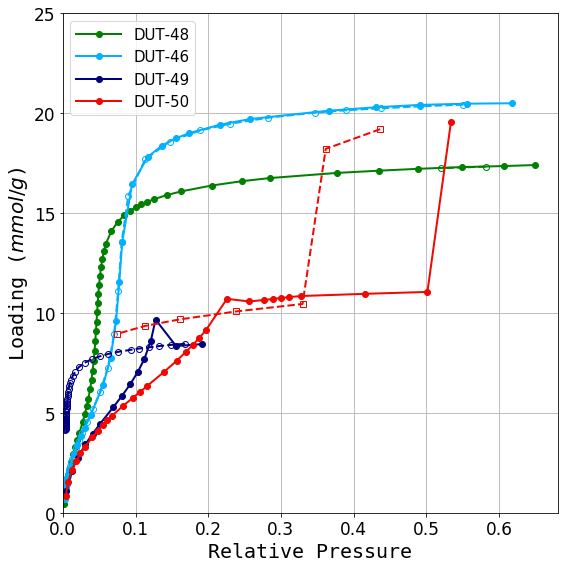
\includegraphics[width=\linewidth]{butane/dut-reticular-reg}%
        \caption{}\label{dut:fgr:dut-reticular-reg}
    \end{subfigure}%
    \begin{subfigure}{0.33\linewidth}
        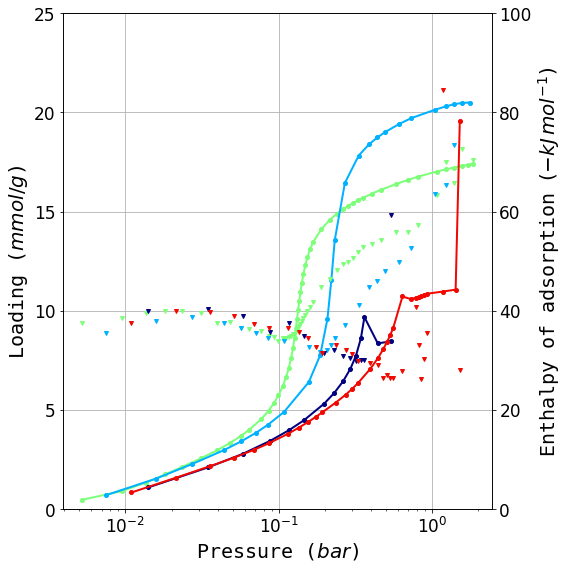
\includegraphics[width=\linewidth]{butane/dut-reticular-log}%
        \caption{}\label{dut:fgr:dut-reticular-log}
    \end{subfigure}%
    \begin{subfigure}{0.33\linewidth}
        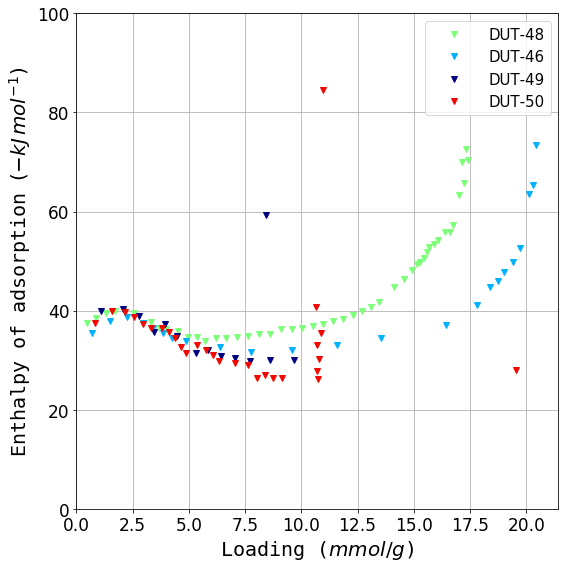
\includegraphics[width=\linewidth]{butane/dut-reticular-enth}%
        \caption{}\label{dut:fgr:dut-reticular-enth}
    \end{subfigure}%
    \caption{Estimated errors at a 95\% confidence range for 
    (a) loading as a function of pressure, 
    (b) differential enthalpy as a function of pressure 
    (c) differential enthalpy as a function of loading.}%
    \label{dut:fgr:dut-reticular}
\end{figure}

\begin{figure}[htb]
    \centering
    \begin{subfigure}{0.5\linewidth}
        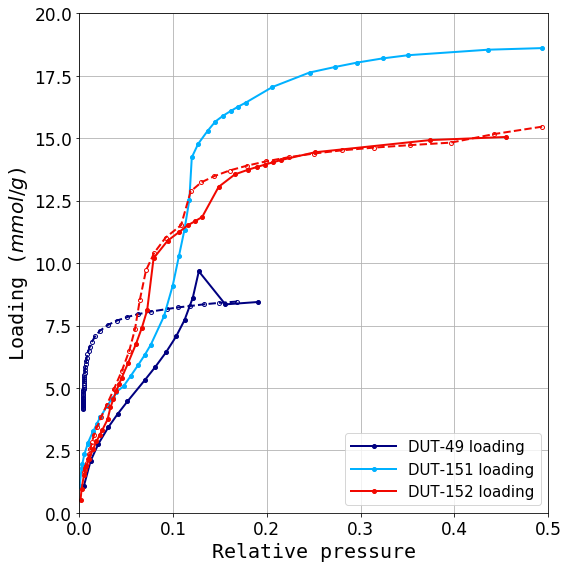
\includegraphics[width=\linewidth]{butane/dut-reticular-interp-reg}%
        \caption{}\label{dut:fgr:dut-reticular-interp-reg}
    \end{subfigure}%
    \begin{subfigure}{0.5\linewidth}
        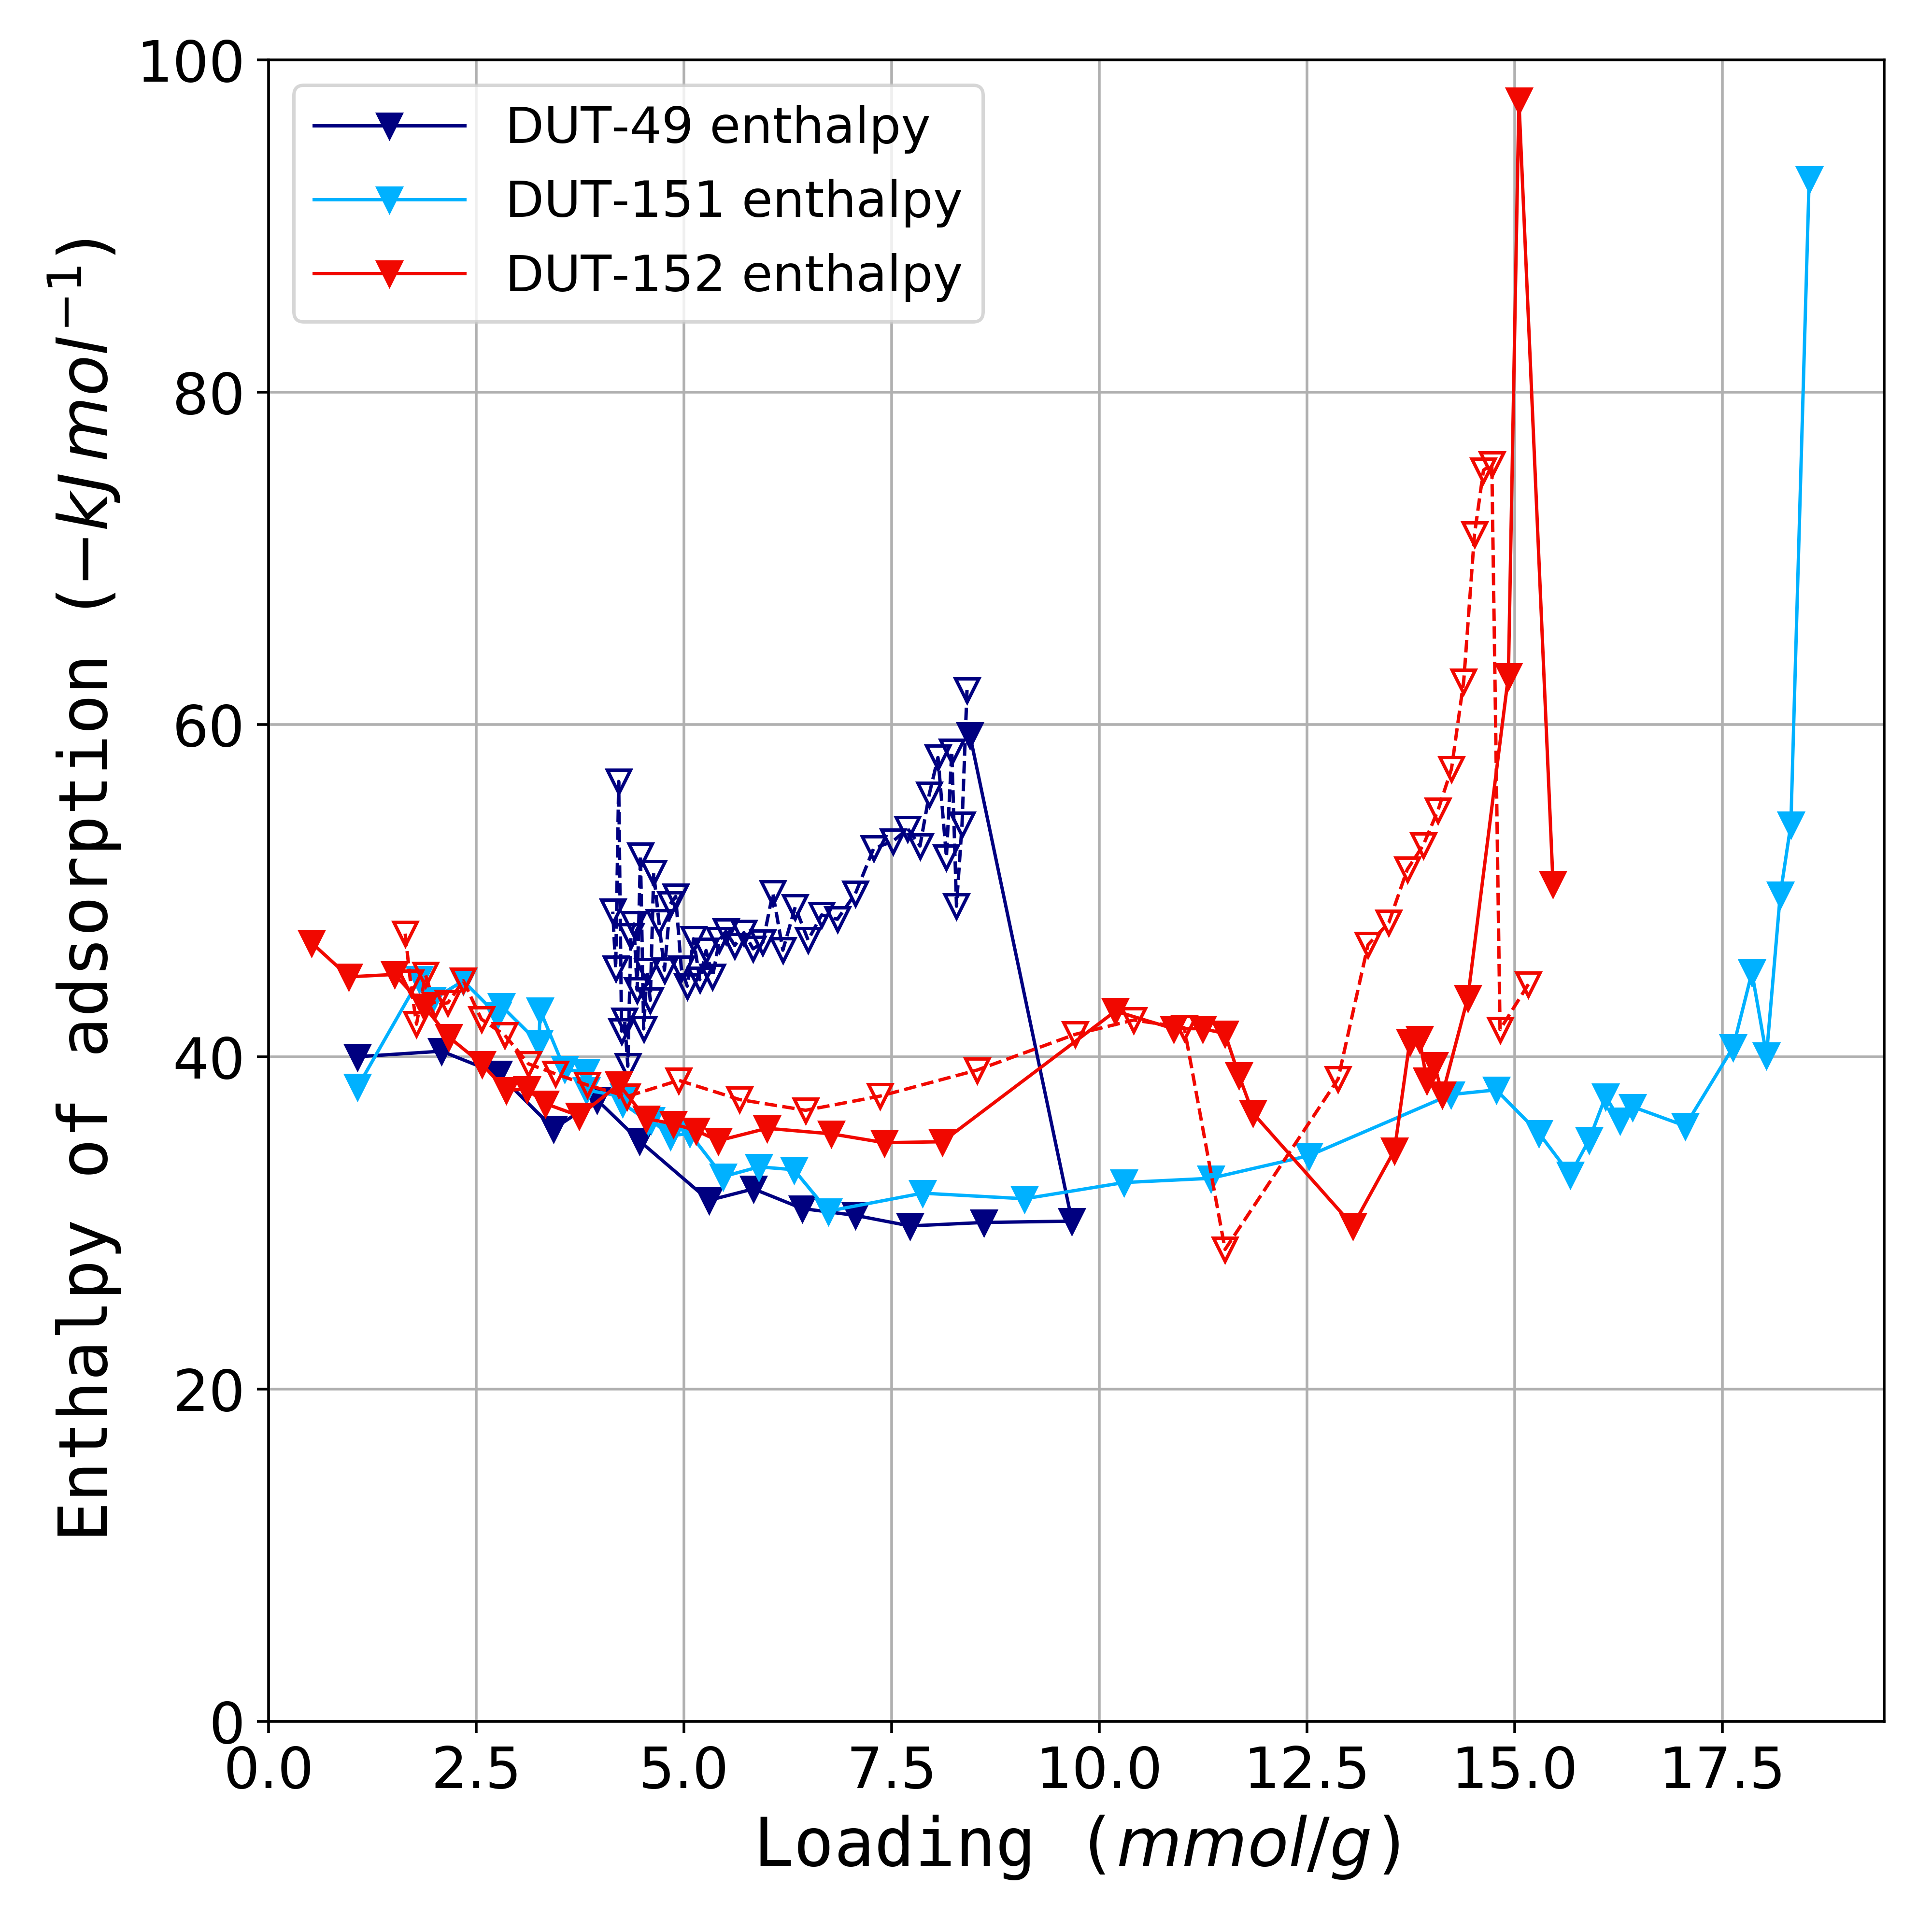
\includegraphics[width=\linewidth]{butane/dut-reticular-interp-enth}%
        \caption{}\label{dut:fgr:dut-reticular-interp-log}
    \end{subfigure}%
    \caption{The (a) isotherms and (b) enthalpy curves of the
    interpenetrated materials DUT-151 and DUT-152. Shaded regions
    are guides for the eye.}%
    \label{dut:fgr:dut-reticular}
\end{figure}